\documentclass[tikz,border=2pt]{standalone}

\usetikzlibrary{arrows.meta,decorations.pathreplacing}

\begin{document}

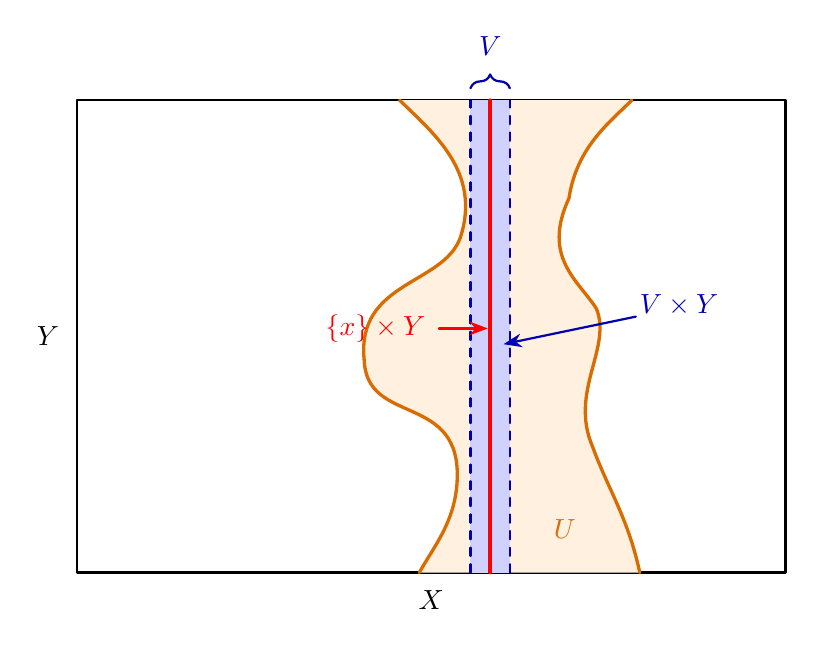
\begin{tikzpicture}[
    >=Stealth,
    line cap=round,
    line join=round
]

% Ambient space X x Y
\draw[thick] (0,0) rectangle (9,6);

% Labels for X and Y
\node[below] at (4.5,-0.1) {$X$};
\node[left]  at (-0.1,3) {$Y$};

% The open set U (orange region)
\fill[orange!12]
    (4.1,6)
    .. controls (4.5,5.6) and (5.15,5.1) .. (4.87,4.25)
    .. controls (4.65,3.65) and (3.55,3.7) .. (3.65,2.7)
    .. controls (3.68,1.85) and (4.9,2.3) .. (4.83,1.15)
    .. controls (4.8,0.65) and (4.55,0.35) .. (4.35,0)
    -- (7.15,0)
    .. controls (7.0,0.7) and (6.75,1.05) .. (6.55,1.6)
    .. controls (6.25,2.3) and (6.8,2.85) .. (6.6,3.35)
    .. controls (6.38,3.7) and (5.9,4.0) .. (6.25,4.75)
    .. controls (6.35,5.4) and (6.75,5.7) .. (7.05,6)
    -- cycle;

% Left boundary of U
\draw[orange!85!black,very thick]
    (4.1,6)
    .. controls (4.5,5.6) and (5.15,5.1) .. (4.87,4.25)
    .. controls (4.65,3.65) and (3.55,3.7) .. (3.65,2.7)
    .. controls (3.68,1.85) and (4.9,2.3) .. (4.83,1.15)
    .. controls (4.8,0.65) and (4.55,0.35) .. (4.35,0);

% Right boundary of U
\draw[orange!85!black,very thick]
    (7.15,0)
    .. controls (7.0,0.7) and (6.75,1.05) .. (6.55,1.6)
    .. controls (6.25,2.3) and (6.8,2.85) .. (6.6,3.35)
    .. controls (6.38,3.7) and (5.9,4.0) .. (6.25,4.75)
    .. controls (6.35,5.4) and (6.75,5.7) .. (7.05,6);

% Product neighbourhood V x Y (blue strip)
\fill[blue!18] (5.0,0) rectangle (5.5,6);

% Boundaries of the blue strip
\draw[blue!70!black,thick,dashed] (5.0,0) -- (5.0,6);
\draw[blue!70!black,thick,dashed] (5.5,0) -- (5.5,6);

% The slice {x} x Y (red line)
\draw[red,very thick] (5.25,0) -- (5.25,6);

% Brace indicating V
\draw[
    blue!70!black,
    thick,
    decorate,
    decoration={brace,amplitude=5pt}
]
    (5.0,6.15) -- (5.5,6.15)
    node[midway,above=8pt] {$V$};

% Label for {x} x Y
\node[red,anchor=east] at (4.55,3.1)
    {$\{x\}\times Y$};

\draw[red,->,thick]
    (4.6,3.1) -- (5.22,3.1);

% Label for V x Y
\node[blue!70!black] at (7.65,3.4)
    {$V\times Y$};

\draw[blue!70!black,->,thick]
    (7.1,3.25) -- (5.42,2.9);

% Label for U
\node[orange!85!black] at (6.2,0.55)
    {$U$};

\end{tikzpicture}

\end{document}